\documentclass[12pt]{article}

\usepackage{array}
\usepackage{amsmath}
\usepackage{amssymb}
\usepackage{mathtools}
\usepackage{textcomp}
\usepackage{gensymb}
\usepackage{graphicx}
\usepackage{float}
\usepackage{caption}
\usepackage{amsfonts}
\usepackage[margin=1in]{geometry}
\newcounter{results}
\newcounter{questions}

\def\neg{{\sim}}
\def\Z{\mathbb{Z}}
\def\N{\mathbb{N}}
\def\R{\mathbb{R}}
\def\Q{\mathbb{Q}}
\def\E{\mathbb{E}}
\def\qed{\(\blacksquare\)}
\newcommand{\result}[1]{\stepcounter{results}{\bfseries Result \arabic{results}}: #1}
\newcommand{\question}[1]{\stepcounter{questions}{\bf \arabic{questions}}: #1}
\newenvironment{proof}[2][Proof]{\result{#2}\begin{trivlist} 
    \item[\hskip \labelsep {\sc #1:}]}{\qed\end{trivlist}}

\begin{document}
    \title{Typesetting in \LaTeX}
    \author{Ryan Coyne}
    \date{}
    \maketitle
    \noindent\textbf{Problem 1.}\\
    Euler's formula, given by \(e^{ix}=\cos x + i\sin x\), establishes the fundamental relationship between the trigonometric functions and the complex exponential function.\\
    \textbf{Problem 2.}
    \begin{align*}
        \int_{T_0}^{T_1} x^2 dx = \frac{1}{3}(T_1^3-T_0^3)
    \end{align*}
    \textbf{Problem 3.}
    \begin{equation}
        \delta x=\sqrt{\frac{1}{N(N-1)}\sum_{i=1}^N(x_i-\overline{x})^2}
    \end{equation}
    \textbf{Problem 4.}
    \begin{table}[H]
        \centering
        \begin{tabular}{|c|c|}
            \hline
            \multicolumn{2}{|c|}{DMM Uncertainties}\\
            \hline
            DMM Model & MASTECH MS82268\\
            \hline
            Resistance: &\(\delta R=(1.2\%\) of rdg + 2 digits)\\
            \hline
            DC Voltage: & \(\delta R= (0.7\% \) of rdg + 2 digits)\\
            \hline
            DC Current: & \(\delta R= (1.2\% \) of rdg + 3 digits)\\
            \hline
        \end{tabular}
    \end{table}
    \noindent\textbf{Problem 5.}
    \begin{figure}[H]
        \centering
        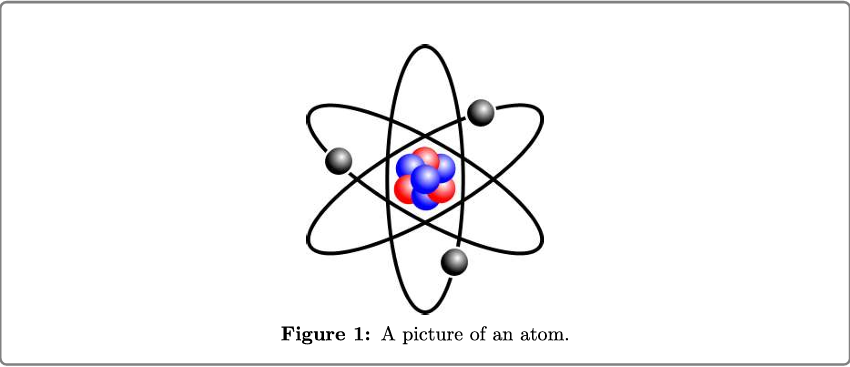
\includegraphics[width=0.8\linewidth]{atom.png}
    \end{figure}
\end{document}